\documentclass[12pt,a4paper]{article}

\usepackage{style2017}
\usepackage{hyperref}

\hypersetup{
    colorlinks =false,
    linkcolor=blue,
   linkbordercolor = 1 0 0
}
\newcounter{numexo}
\setcellgapes{1pt}

\begin{document}



\begin{NSI}
{Activité}{Type de données structuré - les listes}
\end{NSI}

%\textbf{Rappel :} les tableaux en python sont appelés des listes.

%\addtocounter{numexo}{1}
\subsection*{\Large Introduction}

En informatique et en mathématiques, certaines données sont multiples comme les coordonnées d'un point dans un repère avec l'abscisse et l'ordonnée.\medskip

On représente ces données avec des \textbf{tableaux}. Une variable peut contenir plusieurs valeurs contenues dans un tableau.

Prenons l'exemple des notes d'un élève dans une discipline. Il est nécessaire de pouvoir accéder à toutes les notes à tout moment. De pouvoir modifier une valeur, en ajouter, en supprimer et même de les trier...
\bigskip

\subsection*{Notations des listes}
En python, les tableaux sont représentés par des listes. Ces \textsf{listes} regroupent les valeurs séparées par des virgules, le tout entre crochets:
\textsf{[\text{1\up{ère} valeur},~\text{2\up{ème} valeur}, ...,~\text{dernière valeur}]}

%Une variable de type liste contient une liste de valeurs comme valeur! Par exemple :
%$$T=[\text{1\up{ère} valeur},~\text{2\up{ème} valeur}, ...,~\text{dernière valeur}]$$

Les valeurs d'une liste sont repérées par un \textsf{indice}. La première valeur a pour indice $0$, la seconde valeur a pour indice $1$, etc. Ces indices permettent d'accéder facilement aux valeurs de la liste.

\subsection*{Fonctions et méthodes sur les listes}

Certaines \textbf{fonction}s et \textbf{méthodes} sont disponibles pour différents types de données et d'autres sont spécifiques aux listes.\medskip

\subsubsection*{Les fonctions}
\begin{itemize}
\item La fonction \textsf{len} renvoie le nombre de valeurs dans la liste: on l'appelle longueur de liste.
\item La fonction \textsf{min} renvoie la plus petite valeur de la liste lorsqu'elles sont numériques.
\item La fonction \textsf{max} renvoie la plus grande valeur de la liste lorsqu'elles sont numériques.
\item La fonction \textsf{sum} calcule et renvoie la somme des valeurs de la liste si elles sont numériques.
\end{itemize}


\subsubsection*{Les méthodes}
\begin{itemize}
\item La méthode \textsf{index} renvoie l'indice (position) d'une valeur de la liste.
\item La méthode \textsf{append} ajoute une nouvelle valeur en fin de liste.
\item La méthode \textsf{pop} supprime et renvoie la valeur à l'indice donné.
\item La méthode \textsf{sort} trie la liste des valeurs par ordre croissant.
\end{itemize}

\textbf{Attention !} une méthode se place derrière une variable séparée par un point.\medskip


\newpage
\addtocounter{numexo}{1}
\subsection*{\Large Partie \thenumexo}

Un élève a eu 6 notes, toutes évaluées sur 20, depuis le début de l'année. 

On crée un tableau contenant toutes les notes affecté à la variable \textsf{notes}
: \textsf{notes=[13, 7, 11, 18, 9, 12]}

\begin{enumerate}
\item Quel est le type de la variable \textsf{notes}? \vspace{1.5cm}

\item Quelle est la valeur de \textsf{notes[2]} ? \vspace{1.5cm}

\item Comment obtenir la première et la dernière note du tableau? \vspace{3cm}

\item Notre élève a une note supplémentaire : 15. Comment l'ajouter à la liste ? \vspace{3cm}

\item Comment connaitre le nombre de notes ? La note la plus haute ? La plus faible ? \vspace{3cm}
\end{enumerate}

\newpage
\addtocounter{numexo}{1}
\subsection*{\Large Partie \thenumexo }
\begin{enumerate}
\item On donne le code suivant:
\begin{center}
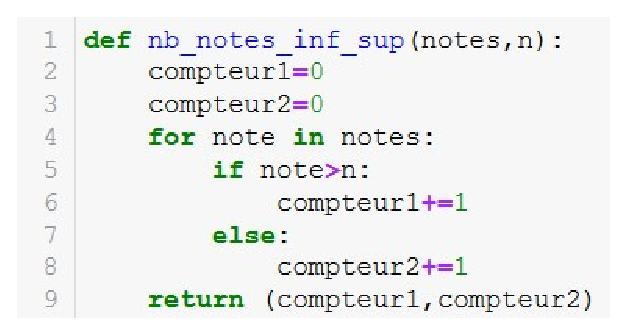
\includegraphics[scale=0.8]{img/algo1.eps}
\end{center}
\begin{enumerate}
\item Quel est le type de retour de cette fonction ? \vspace{1cm}

\item Quelle est la valeur obtenue à l'appel \textsf{nb\_notes\_inf\_sup(notes,10)} ?\vspace{1cm}
\end{enumerate}

\item En statistiques, on appelle \textsf{étendue}, la différence entre la plus grande et la plus petite valeur de la série de notes. 

Écrire la fonction \textsf{etendue} prenant en paramètre la liste de notes et renvoyant l'étendue de la liste. \vspace{4cm}

\item La moyenne d'une série de notes se calcule par la somme de toutes les notes divisée par le nombre de notes. 

Écrire la fonction \textsf{note\_moy} qui prend en paramètre la liste de notes et renvoie la moyenne des notes de l'élève. \vspace{4cm}

\item La médiane d'une série de notes est la note qui a autant de valeurs inférieures que de valeurs supérieures. On tient compte de la parité du nombre de notes.

Écrire la fonction \textsf{mediane} qui prend en paramètre la liste notes, et renvoie la note médiane.
\end{enumerate}

\newpage
\addtocounter{numexo}{1}
\subsection*{\Large Partie \thenumexo }
Dans cette partie, les notes ont des coefficients. On va donc créer une liste dont chaque valeur est une liste constituée de la note et du coefficient. 

Par exemple, un candidat a eu les notes suivantes à un examen:
\begin{itemize}
\item français: 12, coefficient : 4
\item mathématiques: 13, coefficient : 5
\item anglais: 9, coefficient : 2
\item histoire: 14, coefficient : 2
\item sciences: 11, coefficient : 3
\end{itemize}
La liste des notes est alors:
$$\text{notes}=[~[12,4],[13,5],[9,2],[14,2],[11,3]~]$$
\begin{enumerate}
\item \begin{enumerate}
\item Quelle est la valeur de \textsf{notes[1]}? \vspace{2cm}

\item Comment obtient-on la valeur et le coefficient de la troisième note ?\vspace{2cm}

\end{enumerate}

\item Écrire une boucle qui affiche seulement les notes. Seulement les coefficients. \vspace{4cm}

\item Écrire la fonction \textsf{moy\_coef} qui prend en paramètre la liste de notes et renvoie la moyenne.


\end{enumerate}

\end{document}

